\chapter{Image Processing Techniques} % Chapter 3
%

%\nocite{*}

\section{Introduction} % a.
This chapter looks at image processing techniques used in obtaining the features needed to do the final classification. The Viola and Jones algorithm, developed by Viola and Jones, is used to detect the location of the frontal face in the image. Once we have this location we then extract the face, which represents our region of interest. The region of interest is then Gray-scaled and is now ready for feature extraction. The Histogram of Oriented Gradients(HOG) is used for the feature extraction process. 

The rest of this chapter is organised as follows: Section 3.2 provides details on Viola-Jones Object Detection and it's key concepts; Section 3.3 covers the image pre-processing techniques used and Section 3.4 explains how Histogram of Oriented Gradients are used for feature extraction.

\section{Viola-Jones Object Detection}
\begin{flushleft}
The Viola-Jones algorithm \citep{viola} is an object detection method that uses Haar-like features. For this project the Viola-Jones object detection is used to find the location of frontal faces in images. The algorithm uses three concepts to effectively detect objects with certain features:\\

The first concept is the integral image, which allows for the features in the image to be evaluated much faster. This is also known as an intermediate view of the image. At each point$(x,y)$ in the integral image, there is the sum of the pixels above and to the left of the point$(x,y)$,inclusive.\\
Referring to Figure ~\ref{fig: integral}:
In order to calculate the sum of the pixels within the rectangle D, only four original  image references are needed.

\begin{itemize}
\item At point 1 in the integral image, the sum of all the pixels in rectangle A in the original image are used. 
\item At point 2 in the integral image the sum of all the pixels in rectangles A and B in the original image are added together(A+B). 
\item At point 3 in the integral image the sum of all the pixels in rectangles A and C in the original image are added together(A+C). 
\item Lastly, at point 4 in the integral image of all the rectangles are added together (A+B+C+D)in the original image. 
\end{itemize}
Thus, to get the sum of the pixels in rectangle D will result in 4+1-(2+3).
\end{flushleft}
\begin{figure}[H]
  \centering
  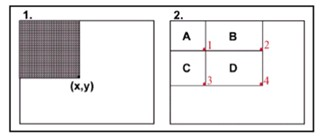
\includegraphics[scale=0.8]{1}
  \caption{Integral Image\citep{viola}}
  \label{fig: integral}
\end{figure}
\begin{flushleft}
The second concept in the Viola-Jones framework\citep{viola} is a classifier based on reducing a large feature set down to a smaller set of important features. This is done by using Ada-Boost. Ada-Boost finds a weak classifier and forces it to depend on a single feature, resulting in a stronger classifier. A weak classifier is selected at each stage of the boosting process, or feature selection process.

The third concept is a method that combines weak classifiers in a rejection cascade. This increases the speed of detection as the focus is now on promising areas of the image. Each stage in the cascade is formed using Ada-Boost. The Viola-Jones algorithm uses many Haar-like features. I will describe Three of these Haar-like features.
\begin{itemize}
  \item Two-rectangle feature - is calculated by subtracting the sum of the pixels of one rectangle from the sum of the other. The rectangles need to be the same size, shape and need to be vertically or horizontally adjacent.
  \item Three-rectangle feature - is calculated by subtracting the sum of the two outside rectangles from the middle rectangle.
  \item Four-rectangle feature - is calculated by subtracting the sum of the pixels of one diagonal pair from the other.
\end{itemize} 
\end{flushleft}
\begin{figure}[H]
  \centering
  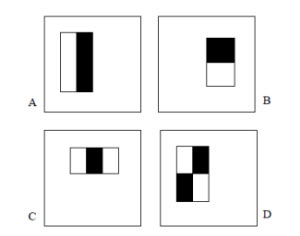
\includegraphics[scale=0.8]{2}
  \caption{Haar-like features\citep{viola}}
\end{figure}

\section{Image Preprocessing}
	\subsection{Resizing} 
	The image is resized once we obtain our region of interest using Viola-Jones to detect the location of the face. The main benefit of resizing the image is to maintain uniformity in our feature set. Another benefit is that it scales down the number of pixels in a image, resulting in a smaller feature set\cite{pre}. 
	\subsection{Gray Scaling}
	Converting an image from RGB(colour) to Grayscale helps in reducing the number of colour channels down to a single color channel. A commonly used method is the standard NTSC conversion formula, that calculates the luminance of a pixel\cite{pre}:

	Luminance of a pixel $= (0.2989 \times red) + (0.5870 \times green) + (0.1140 \times blue) $
	 
\section{Histogram of Oriented Gradients}   
The Histogram of Oriented Gradients is a feature extraction method for images. Where a image is divided into cells, of $C_x \times C_y$ pixels, that form a grid over the image. Histograms are calculated for each of these cells based on the orientation of the gradients of the pixels in the cell. This is followed by the image further being divided into a grid, of $B_x \times B_y$ cells, which are called blocks. Each block is used to contrast-normalize the histograms(cells) present in the block. The dimensions of the final feature vector calculated by: 

$\textrm{total number of blocks} \times \textrm{number of cells in each block} \times \textrm{number of orientation bins}$
\begin{flushleft}
Further details of the Histogram of Oriented Gradients will be discussed following Dalal \& Triggs HOG feature extraction chain,see Figure ~\ref{fig:hhog}, excluding the linear SVM and classification\cite{hog}.
\end{flushleft}
\begin{figure}[H]
  \centering
  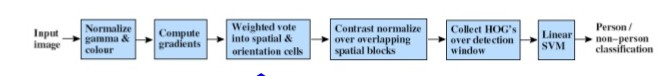
\includegraphics[scale=0.6]{chain}
  \caption{HOG feature extraction chain\cite{hog}}
  \label{fig:hhog}
\end{figure}

\subsection{Input Image}
Given an image, first identify the region of interest in the image. This region then forms your image window.
\begin{figure}[H]
\centering
\begin{minipage}{.5\textwidth}
  \centering
  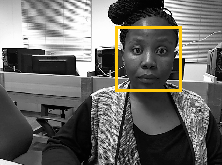
\includegraphics[width=.4\linewidth]{image}
  \captionof{figure}{Region of interest}
  \label{fig:test1}
\end{minipage}%
\begin{minipage}{.5\textwidth}
  \centering
  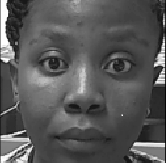
\includegraphics[width=.4\linewidth]{roi}
  \captionof{figure}{Image window}
  \label{fig:test2}
\end{minipage}
\end{figure}
\subsection{Normalize Gamma \& Colour}
Normalizing the image window is an optional addition to the HOG. Dalal \& Triggs found that normalizing the image pixels(p) at this the stage did not have a noticeable impact on the performance at the detection stage of their research.
However when choosing to normalize the image window Gamma (power law) normalization had a negative impact on the results, while Square-root normalization had more of a positive impact on the results.

Gamma Normalization: $log_(p)$ 

Square-root Normalization: $\sqrt{p}$
\subsection{Gradients}
The gradient for the image window is computed by applying a one dimensional mask in both X ($G_x$) and Y ($G_y$) directions.\

\begin{figure}[H]
  \centering
  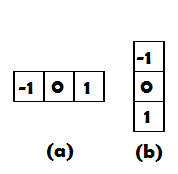
\includegraphics[scale=0.8]{sobel}
  \caption{One dimentional masks,(a)X-direction and (b) Y-direction}
\end{figure}
\begin{flushleft}
The mask convolves over the image window. At each point where the mask is placed the pixels are multiplied by the mask. After that the two outer pixels are added together and the result is placed in the position of the center pixel. The mask is not able to compute the gradients on the pixels around the egde of the image. Unless extra pixels are added to the edges of the image before hand. The example below shows how the loss in pixels affects the resulting gradient image.
\end{flushleft}
\subsubsection{Example:}

\begin{figure}[H]
\centering
\begin{subfigure}{.5\textwidth}
  \centering
  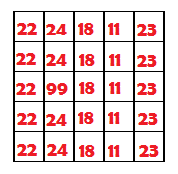
\includegraphics[width=.4\linewidth]{im}
  \label{fig:sub1}
\end{subfigure}%
\begin{subfigure}{.5\textwidth}
  \centering
  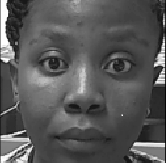
\includegraphics[width=.4\linewidth]{roi}
  \label{fig:sub2}
\end{subfigure}
\caption{Image window}
\label{fig:test}
\end{figure}
\begin{figure}[H]
\centering
\begin{subfigure}{.5\textwidth}
  \centering
  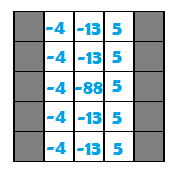
\includegraphics[width=.4\linewidth]{gx}
  \label{fig:sub1}
\end{subfigure}%
\begin{subfigure}{.5\textwidth}
  \centering
  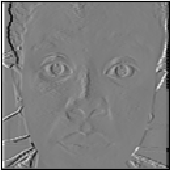
\includegraphics[width=.4\linewidth]{dx}
  \label{fig:sub2}
\end{subfigure}
\caption{The result of a one dimensional mask applied in the X-direction}
\label{fig:test}
\end{figure}
\begin{figure}[H]
\centering
\begin{subfigure}{.5\textwidth}
  \centering
  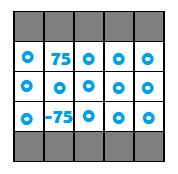
\includegraphics[width=.4\linewidth]{gy}
  \label{fig:sub1}
\end{subfigure}%
\begin{subfigure}{.5\textwidth}
  \centering
  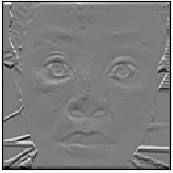
\includegraphics[width=.4\linewidth]{dy}
  \label{fig:sub2}
\end{subfigure}
\caption{The result of a one dimensional mask applied in the Y-direction}
\label{fig:test}
\end{figure}


Now that we have the gradients, we can compute the magnitude and orientation of the gradients from  $G_x$ \& $G_y$.

Magnitude: $G = \sqrt{G_x + G_y}$

Orientation: $\theta = arctan(\dfrac{G_y}{G_x})$

\subsection{Weighted Vote in Spatial \& Oriented Cells}
We can now decide on the dimensions of each cell, before calculating the HOGs. In their research Dalal \& Triggs found that the size of the cell are dependent on the size of the features you need to extract(e.g eyes, nose, mouth). 
\begin{figure}[H]
\centering
\begin{minipage}{.5\textwidth}
  \centering
  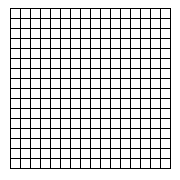
\includegraphics[width=.4\linewidth]{pixels}
  \captionof{figure}{$16 \times 16$ pixel image}
  \label{fig:test1}
\end{minipage}%
\begin{minipage}{.5\textwidth}
  \centering
  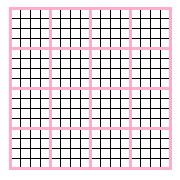
\includegraphics[width=.4\linewidth]{cells}
  \captionof{figure}{Image divided into $4 \times 4$ pixel cells}
  \label{fig:test2}
\end{minipage}
\end{figure}
The next parameter is the number of orientation bins. The orientation of the gradient can be described as the angle of the gradient. There are two options available when choosing the range of the gradient angle:
\begin{itemize}
  \item Signed [0,360] degrees
  \item Unsigned [0,180] degrees
\end{itemize}
Unsigned gradients in the range [0,180] degrees, with the number of orientation bins in the range [9,12] are the preferred values for the orientation bins.
\begin{figure}[H]
\centering
\begin{minipage}{.5\textwidth}
  \centering
  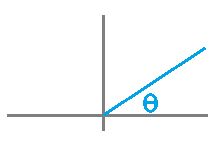
\includegraphics[width=.4\linewidth]{theta}
  \captionof{figure}{$\theta$ as an angle}
  \label{fig:test1}
\end{minipage}%
\begin{minipage}{.5\textwidth}
  \centering
  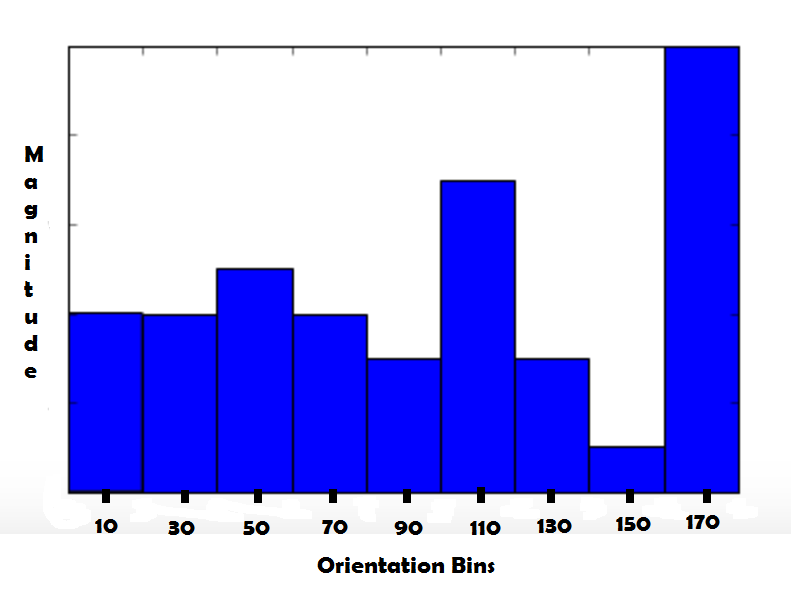
\includegraphics[width=.4\linewidth]{hist}
  \captionof{figure}{Unsigned gradients with 9 orientation bins}
  \label{fig:test2}
\end{minipage}
\end{figure}
Looking at a single cell. Each pixel of the gradient magnitude image contributes to a orientation bin of a cells histogram. The value of the same pixel in the gradient orientation image helps you identify which orientation bin to place the gradient magnitude of the pixel.

\subsection{Contrast Normalize over Overlapping spatial cells}
Contrast normalization is used to ensure that the cells are not affected vastly by changes illumination and contrast in the image. Starting with dividing the image into blocks that can fit at least 2-3 features, these blocks are allowed to overlap one another for more detailed feature set. Contrast normalization works by taking the sum of the histograms in a block $S_b$ and dividing each of the histograms $H_{hist}$ by $\sqrt{S_b ^2 + \epsilon ^2}$. The result is a normalized histogram $H_{norm}$ in each cell. 

Contrast normalization : $H_{norm} = \dfrac{H_{hist}}{\sqrt{S_b  ^2 + \epsilon ^2}}$
\begin{figure}[H]
\centering
\begin{minipage}{.5\textwidth}
  \centering
  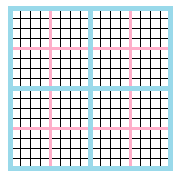
\includegraphics[width=.4\linewidth]{blocks}
  \captionof{figure}{Blocks of $B_x \times B_y$ cells}
  \label{fig:test1}
\end{minipage}%
\begin{minipage}{.5\textwidth}
  \centering
  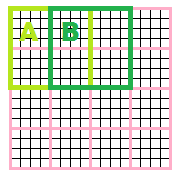
\includegraphics[width=.4\linewidth]{overlap}
  \captionof{figure}{Block A \& B with a 50\% overlap}
  \label{fig:test2}
\end{minipage}
\end{figure}

\begin{figure}[H]
  \centering
  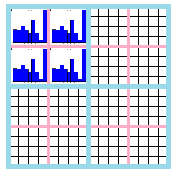
\includegraphics[scale=0.8]{norm}
  \caption{Cell histograms for contrast normalization in a block}
\end{figure}

\subsection{Collect HOGs over Detection Window}
The final step is to concatenate all the normalized histograms to form a one dimensional feature vector $[H_{norm}, H_{norm}, H_{norm}...]$. This feature vector is then used for the classification and training of the system.

